\renewcommand{\chaptername}{\scshape Partie}
\chapter{\normalfont \scshape Effet Schlieren}
\section{Principe du dispositif}
L'air est un fluide transparent, il possède un indice de réfraction qui suit une évolution linéaire par rapport à la densité :
\begin{align}
	n = 1\,+\,k\,\rho
\end{align}
où $\mathnormal{n}$ est l'indice de réfraction du fluide, $\mathnormal{\rho}$ sa densité et $\mathnormal{k}$ une constante appelée constante de Gladstone-Dale~\ref{ref:harvardedu}. Si $\mathnormal{n_i}$ et $\mathnormal{n_r}$ sont respectivement les indices de réfraction des rayons incident et réfléchi, $\mathnormal{\theta_i}$ l'angle d'incidence et $\mathnormal{\theta_r}$ l'angle de réfraction, on peut écrire la loi de Snell-Descartes :
\begin{align}
	n_i\times\,sin(\theta_i) = n_r\times\,sin(\theta_r) 
\end{align}
En faisant varier de manière non uniforme la température ou la pression de l'air, on fait apparaître des gradients de densité, ce qui fait que l'indice de réfraction ne varie pas de la même façon partout dans le fluide. Par conséquent, les rayons lumineux sont déviés, ce qui permet d'observer l'effet Schlieren.
\subsection{Dispositif avec miroir sphérique}
\subsection{Dispositif avec lentilles convergentes}
\section{Protocole et organisation}
\subsection{Cahier des charges}
Une fois l'objectif de cette partie défini, la mise en place d'un plan d'organisation s'est avérée judicieuse pour avancer dans le projet. Pour ce faire, le diagramme de GANTT de la figure~\ref{fig:gantt_schlieren} a été établi :
\begin{figure}[H]
	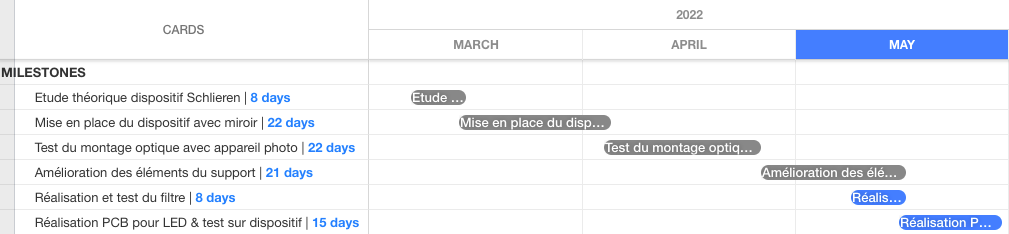
\includegraphics[scale = 0.43]{figures/gantt_schlieren.png}
	\caption{\small{\textit{Diagramme de GANTT prévu pour le montage optique}}}
	\label{fig:gantt_schlieren}
\end{figure}
Par ailleurs, parmi les sept membres du groupe, quatre ont été chargés de mettre en place le système optique, un rôle a été attribué à chacun des membres :
\begin{table}[H]
	\centering
	\setlength{\tabcolsep}{15pt}
	\begin{tabular}{|l l l l|}
		\hline
		\vtop{\hbox{\strut \small\textbf{Responsable}}\hbox{\strut \small\textbf{effet Schlieren}}}&\vtop{\hbox{\strut \small\textbf{Responsable}}\hbox{\strut \small\textbf{communication}}}&\vtop{\hbox{\strut \small\textbf{Responsable}}\hbox{\strut \small\textbf{technique}}}&\vtop{\hbox{\strut \small\textbf{Responsable}}\hbox{\strut \small\textbf{planning}}}\\
		\hline
		\vtop{\hbox{\strut \small{Yvonne}}\hbox{\strut \small{SAUTRIOT}}}&\vtop{\hbox{\strut \small{Léo}}\hbox{\strut \small{LAFFAY}}}&\vtop{\hbox{\strut \small{Alexandre}}\hbox{\strut \small{OCKIER}}}&\vtop{\hbox{\strut \small{Nada}}\hbox{\strut \small{KOUDDANE}}}\\
		\hline
	\end{tabular}
	\caption{\small\textit{Membres et tâches attribuées (dispositif à imagerie Schlieren)}}
	\label{fig:gestion_schlieren}
\end{table}
\subsection{Mise en place des montages optiques}

\subsection{Améliorations des montages}
\section{Observations et conclusion}
\subsection{Description des résultats}
\subsection{Interprétation}
\subsection{Conclusion partielle}